\section{\label{sec:level1}CSAC Research and Development}
%In addition, DR absorption $\gamma$ is larger than the CPT transmission %peak due Doppler and pressure broadening such that the overall absorption %for CPT and DR is an approximately Gaussian function yet the CPT %transmission feature is approximately Lorentzian.. 

%The DARPA CSAC outcomes from the main contributors and the other impactful research contributing to meeting the ultimate goal of producing a robust miniaturised atomic clock is examined 

%. Additionally, the current CSAC research and the future outlook following the launch of DAPRA's ACES is discussed in this section. 

\begin{figure}[b]
\centering
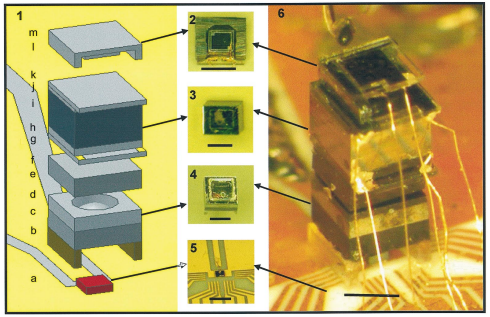
\includegraphics[height=0.27\textwidth,keepaspectratio]{NISTwafer}
\caption{\label{fig:NISTwafer}NIST CSAC physics package. (1) Schematic components: (a) VCSEL, (b) glass, (c)(d)(e)(f) $\lambda$/4 wave-plate optics, (g) indium-tin oxide (ITO) film, (h) glass, (i) Silicon, (j) glass, (k) ITO film, (l) glass, (m) glass. (2) photodiode, (3) $Cs$ vapor cell, (4) optics, (5) laser and (6) physics assembly where the scaling is shown by the 1mm black line $^[$\citep{Knappe2004AClock}$^]$.}
\end{figure}


Prior to beginning construction of the CSAC model, Symmetricom completed an experimental study of the potential for CPT or the conventional double-resonance (DR) technique, used previously in the Symmetricom X72 oscillator,  to meet the DARPA criteria $^[$\citep{Lutwak2002TheInterrogation}$^]$. The testing MEMS package contained a < 1 mm$^3$ vapour cell. $Cs$ were used due to the increased vapour pressure at the operating temperature $>$ 65 $^{\circ }\textrm{C}$ compared to $Rb$. Despite the CPT method having a resonance $\gamma$ approximately 1/2 that of the conventional method, DR was deemed the better technique to obtain short-term stability. This is due to the 10 times larger DR $S/N$ due to contributions of the carrier and second-order sidebands to the background level for CPT. However, Symmetricom express concern over the microwave cavity of the DR technique being the limiting factor to further reduce size. Symmetricom further investigates using CPT spectroscopy in Ref. [\citen{LutwakRandEmmonsDEnglishTRiley2003TheProgress}] determining that D1 line resonance increases the frequency stability compared to applying the laser field on the D2 line. 

\begin{figure}[b]
\centering
\begin{subfigure}[b]{0.45\textwidth}
   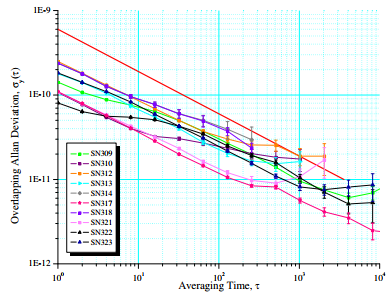
\includegraphics[width=1\linewidth]{shorttermstab}
	\caption{\label{fig:shorttermstab}}
\end{subfigure}
\begin{subfigure}[b]{0.45\textwidth}
   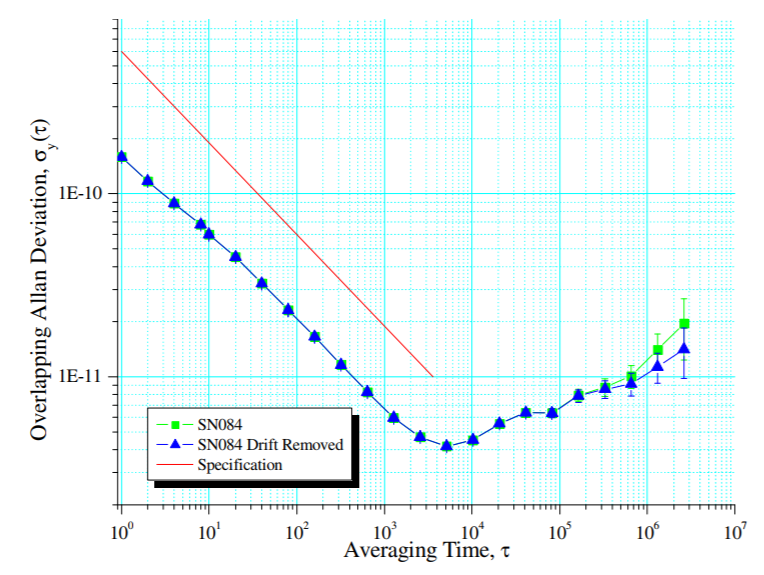
\includegraphics[width=1\linewidth]{longtermstab}
	\caption{\label{fig:longtermstab}}
\end{subfigure}
\caption[]{$\sigma_{y}(\tau$) for (a) short-term and (b) long-term (6 months) measurements where the drift linear component present (removed) in green (blue) $^[$\citep{LutwakR.RashedA.Varghese2007TheEvaluation}$^]$.}
\end{figure}



In 2004 the National Institute of Standards and Technology (NIST) revealed the first CSAC prototype with a 9.5 mm$^3$ volume MEMS fabricated physics package $^[$\citep{Knappe2004AClock}$^,$\citep{Gerginov2005Component-levelReference}$^]$. NIST pioneered the layered wafer structure fabrication of the physics package shown in Fig (\ref{fig:NISTwafer}) which requires 75 mW to operate, uses the CPT method and enables the production of many units at once. Implementation of 1 mm$^3$ $Cs$ vapor cell fabrication proposed by NIST in Ref. [\citen{Kitching2002MiniatureReference}] using anodic bonding of borosilicate glass and silicon (Si), instead of glass blowing techniques, reduces the cell size.  



In Ref. [\citen{Gerginov2005Component-levelReference}] improvements to the NIST physics package included the addition of the thermally isolating baseplate and a lithographic etching in tungsten film on the baseplate provided a heater below the VCSEL. This reduces the power required to operate the VCSEL. The CSAC prototype use a voltage-controlled oscillator (VCO) as the LO and control electronics implemented servo locking of the LO frequency only. The combined volume of physics package, the B-field coils and shielding was 0.7 cm$^{3}$. The CSAC prototype achieves short-term stability ($\tau$<100 s) of $6\times10^{-10}/\sqrt{\tau}$, total power consumption < 200 mW and has a 10 cm$^{3}$ volume.

Thereafter, Symmetricom produced their first prototype in 2005 with short term stability $\approx4\times 10^{-10}/\sqrt{\tau}$, power consumption <200 mW and 10 cm$^{3}$ volume $^[$\citep{LutwakTheClock}$^]$. The physics package was contained in a vacuum sealed ceramic lid to thermally isolate the components for military operation in ambient temperature ranging between -40 $^{\circ }\textrm{C}$ and 85 $^{\circ }\textrm{C}$ $^[$\citep{LutwakTheClock}$^]$. To make the CSAC more robust the the vapor cell is secured by polyimide tethers. To reduce the control electronics components required and thus the power consumption, a microprocessor is implemented with firmware code. Firmware algorithms demodulate and analyse the error signal of the CPT transmission peak to tune the LO.   



In 2007 in Ref. [\citen{LutwakR.RashedA.Varghese2007TheEvaluation}] the physics package assembly is updated from using "folded-optics" to a component assembly which is similar to the design in Fig. (\ref{fig:NISTwafer}). The $Cs$ transmission peak becomes more symmetric by removing reflection of the laser beam in the prior design. A performance study is undertaken of 10 CSACs, each with 125 mW operating power and 15 cm$^{3}$ volume. Shock testing of the CSAC inspects the cell suspension where all tested devices can sustain a shock up to 500g along all axes. The short-term stability of CSACs is shown in Fig. (\ref{fig:shorttermstab}) where the average stability is $\sigma_{y}(\tau$=1 s) < 1.6 $\times 10^{-10}$. In Fig. (\ref{fig:longtermstab}) $\sigma_{y}(\tau$) is measured for 6 months after the devices has already been operating for 6 months and to inspect the 10$^{12}$/day drift effect. Firmware has been updated proving further power and frequency control of the VCSEL using servo algorithms, complete autonomous locking and acquisition of control parameters.   


Development of other industrial CSAC prototypes includes: Honeywell (1.7 cm$^{3}$, 57 mW, $\sigma_{y}(\tau$=1 hour)=5$\times 10^{-12}$) $^[$\citep{Youngner2007AClock}$^]$ and Teledyne Scientific (< 1 mm$^{3}$, < 30 mW, $\sigma_{y}(\tau$=1 hour) < 10$^{-11}$ $^[$\citep{DeNatale2008CompactClock}$^]$. Ref. (\citen{Douahi2007VapourStandard}) explores 1mm$^{3}$ fabrication producing two cavities. One contains the metallic $Cs$ droplet and dispenses $Cs$ atoms to the other irradiates the cavity. The advantage of this process over the typical anodic bonding process is improved control of the cell atmosphere and $Cs$ purity. 

\begin{figure}[b]
\centering
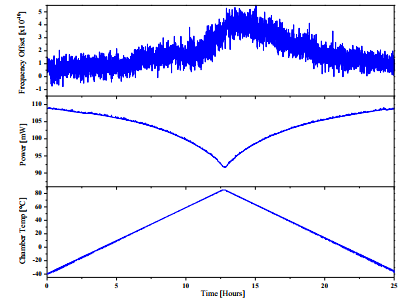
\includegraphics[height=0.32\textwidth,keepaspectratio]{tempplot}
\caption{\label{fig:tempplot}SA.45s performance for chamber temperature ranging between -40 $^{\circ }\textrm{C}$ to 85 $^{\circ }\textrm{C}$.}
\end{figure}

Symmetricom released the SA.45s CSAC commercial product in 2011 with $\sigma_{y}(\tau) < 2\times 10^{-10}/\sqrt{\tau}$, power consumption < 125 mW and volume < 17 cm$^{3}$ $^[$\citep{articleb}$^]$. The CSAC contains: the physics package, 10 MHz TCXO LO, a microprocessor package, a microwave synthesiser mounted on a printed circuit board (PCB). The microwave synethesiser contains the 4.6 GHz VCO which enables modulation of the VCSEL where the VCO is phase-locked to the LO. In addition to the 10 MHz LO output, a 1 pulse-per-second (PPS) output is added for applications requiring GNSS satellite synchronisation. An example of the performance measurements taken in a controlled-temperature environment is shown in Fig. (\ref{fig:tempplot}). The expectation is that low temperatures require more power to temperature control the laser and the vapour cell each with stabilised temperature of 85 $^{\circ }\textrm{C}$ \citep{LutwakR.RashedA.Varghese2007TheEvaluation}. However, the temperature isolation of physics package and efficiency of the electronics reduces the power.

In 2012 Gorecki employed the double cell micro-fabrication technique discussed in Ref. [\citep{Douahi2007VapourStandard}] to produce a CSAC with $\sigma_{y}(\tau$=1 hour) = 5$\times$ 10$^{-11}$, 200 mW power consumption and tens of cm$^{3}$ volume. 




